\section*{Related Work \& Background}

\subsection*{Static Scene Reconstruction}

Before considering scenes with movement or other changing parameters, it's useful to consider scenes where there are no changes.
Static scene reconstruction is the problem of reconstructing a 3D scene from a set of 2D views of a non-changing scene. Neural Radiance Fields (NeRFs)~\cite{mildenhall2020nerf} are a recent technique for reconstructing new views of a scene from unseen camera positions. NeRFs model a scene as a continuous volume of varying density, which has view-dependent color, which allows for representing highly-detailed scenes. NeRF is based on traditional volume rendering techniques:
\begin{align}\label{eq:nerf}
I(r) &= \int_{t_n}^{t_f} T(t, r) \sigma(r(t)) c(r(t), r_d)dt \nonumber \\
T(t, r) &= \exp(-\int_{t_n}^{t} \sigma(r(s))ds)
\end{align}
\noindent
where $I(r)$ is the illumination along camera ray $r(t) = r_o + r_d t$, $r_o, r_d$ are the ray origin and direction respectively, and $t$ is some positive distance along the ray. NeRFs are able to accurately reconstruct high-frequency features by recovering $\sigma,c$, the density and view-dependent color at a given point by modelling them as multi-layer perceptrons (MLPs) with a positional encoding scheme that can differentiate between nearby points in space. NeRFs evaluate the above equations by performing ray-marching and computing $T(j,r) = \sum -\exp\sigma_i c_i$, by partitioning the ray into evenly spaced bins and sampling randomly from within each bin. There has been a plethora of work exploring NeRF and extensions which permit capturing more variance.

These extensions to NeRF include optimizations on the encoding for differentiating positions in space~\cite{tancik2020fourfeat}, better sampling approaches~\cite{barron2021mipnerf}, faster training~\cite{yu2021plenoxels}, and more~\cite{sitzmann2019siren,bi2020neural,srinivasan2020nerv,boss2021nerd}. The underlying canonical model is crucial to our formulation of dynamic NeRF, and for this we use SIREN~\cite{sitzmann2019siren} without a coarse-to-fine approach to get high-frequency details.

\subsection*{Dynamic NeRF Reconstruction}

Dynamic scene reconstruction builds on static scene reconstruction, removing the assumption that all views are under the same condition, such as having the same lighting or that nothing has moved. NeRFs were designed to only handle static scenes, and thus cannot accurately reconstruct scenes which contain movement, alternative lighting conditions, or other changes between frames.
In order to model dynamic scenes, there have been two diverging approaches.

One kind of approach directly models the transformation in the time domain, by learning a function $\sigma(x,t)=f(x\in\mathbb{R}^3, t\in[0,1])$, which include works such as HyperNeRF~\cite{park2021hypernerf}, NeRFies~\cite{park2021nerfies}, Space-Time Invariant Irradiance Fields~\cite{xian2021space}, and others~\cite{Wang_2021_CVPR,du2021nerflow}. By directly modelling the variation of the density, these methods are able to reconstruct large deformations in latent spaces and reconstruct a wide variety of transformations from a single radiance field. These often allow for new transformations in some learned space between similar views, allowing for warping and interpolation between observed views.

The other kind of approach models movement directly as translation, preventing changes in density or view-dependent effects. NeRFs are not able to move the objects inside the scene since we can only evaluate the NeRF at a given $x\in\mathbb{R}^3$. Instead we bend the rays, warping what is visible from a given view. This is essentially a perspective shift of a transformation of the space being rendered: instead of moving an object that should be seen by ray $r$, we warp ray $r$ such that it sees the object. The equation for density is defined as $\sigma(x,t)=f(x+\Delta(x,t))$. This formulation enforces a coherent canonical representation, while directly modelling movement, and has been shown to be able to reconstruct both synthetic scenes with D-NeRF~\cite{pumarola2020dnerf} and real scenes in NR-NeRF~\cite{tretschk2021nonrigid}. There has also been work on recovering movements of multiple NeRFs whose bounding boxes move within a scene, such as in \cite{dynamicSceneGraphs}, but this work diverges from that approach as we are interested in reconstructing movement within one instance of a NeRF.

The benefits of directly including time as a function in the NeRF are that we are able to represent a broader class of functions, in theory every time step or point in latent space may be fully distinct from others, but formulating explicit movement lends itself to smoothness between frames, and accurate reconstruction of the physical process. Our approach falls into the movement category, as we are interested in accurately reconstructing smooth movement as opposed to generalizing over many classes of transformations.

As an aside, we note that a lot of prior work related to dynamic NeRFs have not been peer-reviewed~\cite{pumarola2020dnerf,li2021neural,park2021nerfies,neural3dViewSynthesis}, but these works still have a significant impact, especially since the field moves quickly.

\subsection*{Bezier Curves}
Bezier curves refer to a specific set of polynomials parametrized by a set of control points. They are most commonly represented as cubics: $f(t) = a(1-t)^3 + 3b(1-t)^2t + 3c(1-t)t^2 + dt^3$,
where $t\in[0,1]$ is the variable we are interested in interpolating over, and $a,b,c,d$ are ``control points'' of the function. An example of a Bezier spline (we will use spline and curve interchangeably from here on) is shown in Figure~\ref{fig:bezier_diagram}. The general formulation for
the Bezier basis functions is defined as $B^n(t) = \sum\limits^n_{i=0} {n \choose i} (1-t)^{n-i} t^i$ where $n$
is the degree of the Bezier polynomial. In order to control the Bezier curve, we use control points $P_i$, which control the shape of the curve: $B^n(t) = \sum\limits_{i=0}^n P_i {n \choose i} (1-t)^{n-i} t^i$, where $P_i\in\mathbb{R}^3$ for 3D movement. For a more comprehensive guide on Bezier splines, we refer the reader to a more
\href{https://pomax.github.io/bezierinfo/index.html}{complete reference}~\cite{bezier_primer}\footnote{While this is a not a published, peer-reviewed source, the author found it to be the most well-written, free, and comprehensive resource available.}.

\begin{figure}
    \centering
    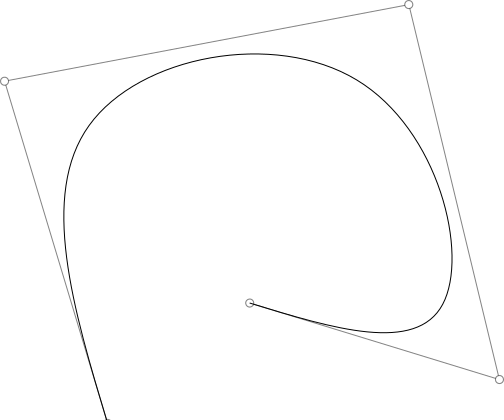
\includegraphics[width=0.2\textwidth]{bezier_curve.png}
    \caption{
        \textbf{Example of a Bezier Spline}.
        Bezier splines are a low-dimensional polynomial for smooth interpolation between a few control points. Our method learns control points to produce smooth movement and induce a prior on continuity, drawing inspiration from animation and drawing software.
    }
    \label{fig:bezier_diagram}
\end{figure}

